\chapter{Descriptors extraction and dimension reduction}
In person re-identification, it's very important to choose robust descriptor to represent person. A good descriptor should be robust to variations of illumination, viewpoint, and camera color response. Most descriptors tries to seize the color and texture information. In this chapter, we will first introduce some basic descriptors and compare their performance on VIPeR dataset, then a detailed introduction of hierarchical descriptor will be presented in the coming section.


\section{Basic color and textural features}
\subsection{Color histogram descriptors on different color space}
Histogram descriptor extracts color statistics information of input images. A popular histogram extracting method is to divide input image into a few horizontal stripes and extract color histogram of each stripe, then they are concatenated to consist of histogram descriptor of the whole image. Color space selection has much influence on descriptor performance. HSV color space is very common used in computer vision and image processing area for target detection and tracking. The HSV descriptor has better performance than RGB histogram descriptor since HSV color separates image intensity from color information. Thus HSV color space is more robust to illumination variation. An unsupervised CMC performance comparison among different color spaces on VIPeR dataset is given in Figure \ref{CMCcolorspaces}. In this comparison camera a views are used as probe set and camera B views are used for gallery set. We can find that those color spaces separating intensity information outperform RGB color space by a large margin.
%-----------------------------------------------------------------------------

\begin{figure}[H]
\centering
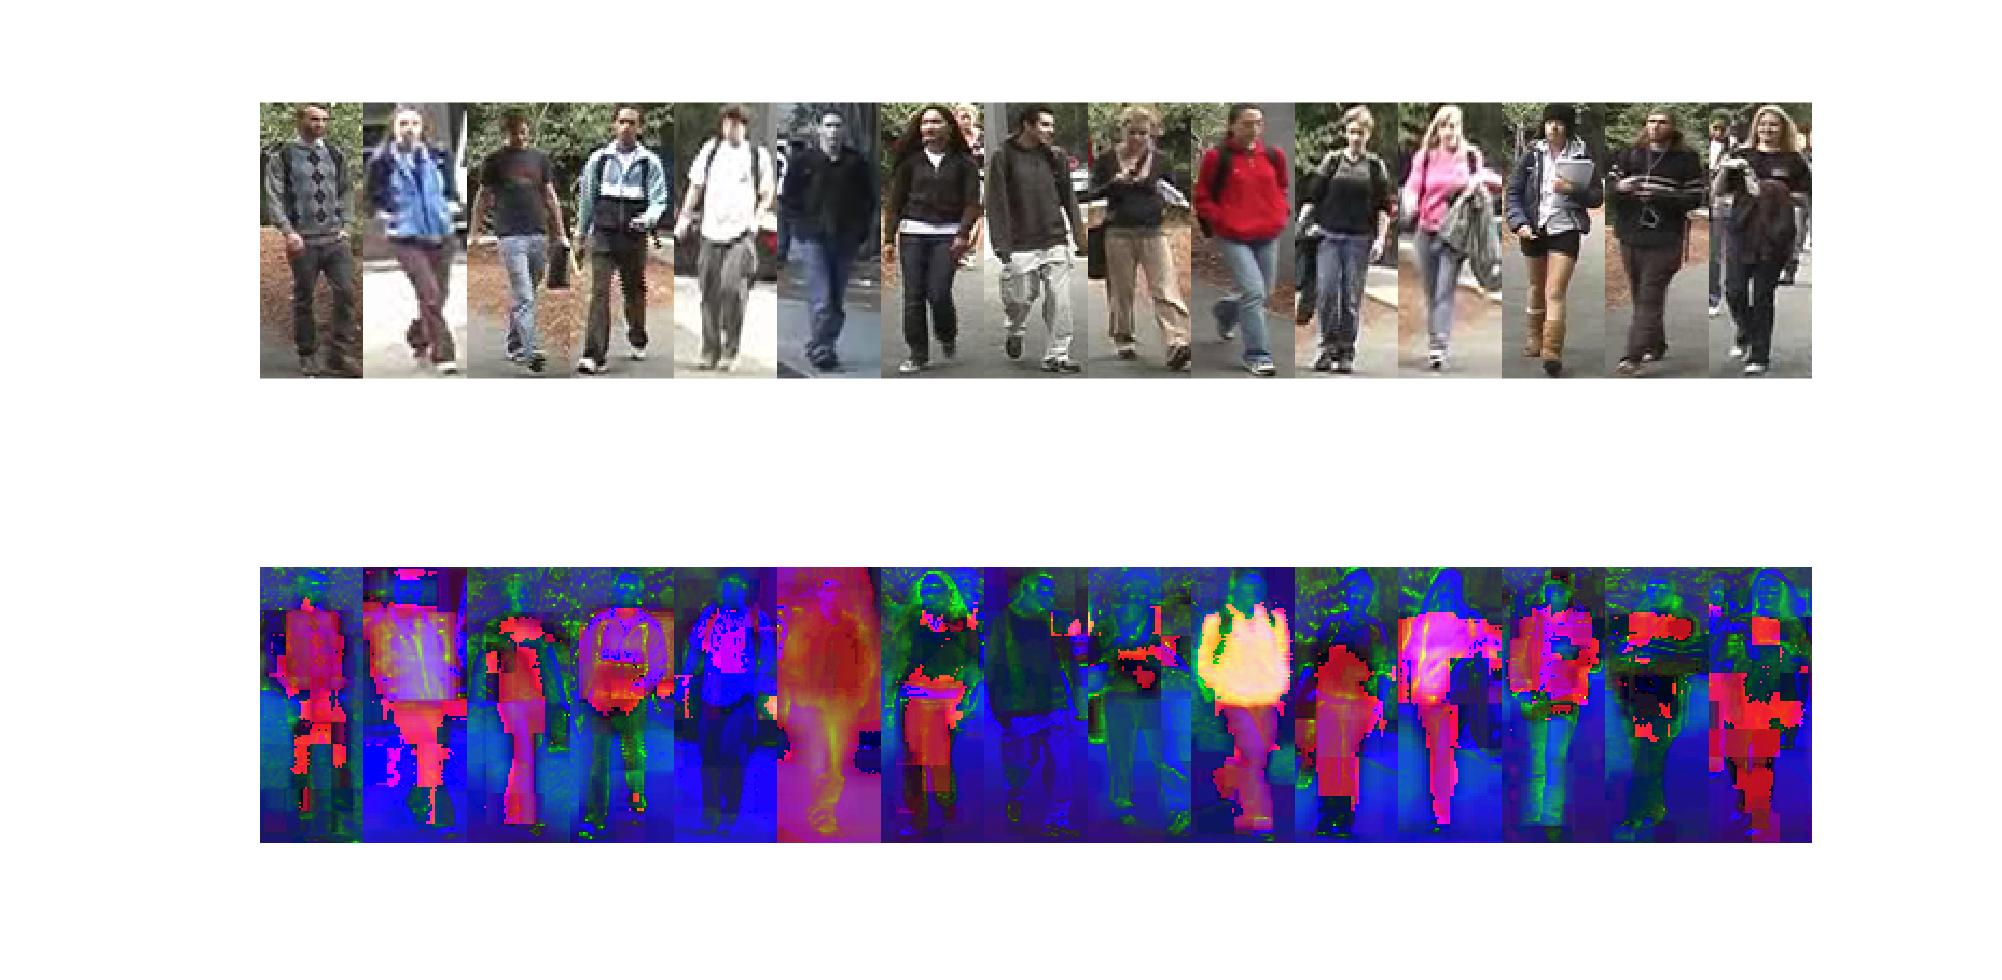
\includegraphics[width=1\linewidth]{/Users/JohnsonJohnson/Downloads/thesis_1/Figures/CompRGBHSV.jpg}
\caption{RGB and HSV visual comparison, the first row is RGB and second row is HSV for same views }
\vspace{0em}
\end{figure} 

\begin{figure}
\centering
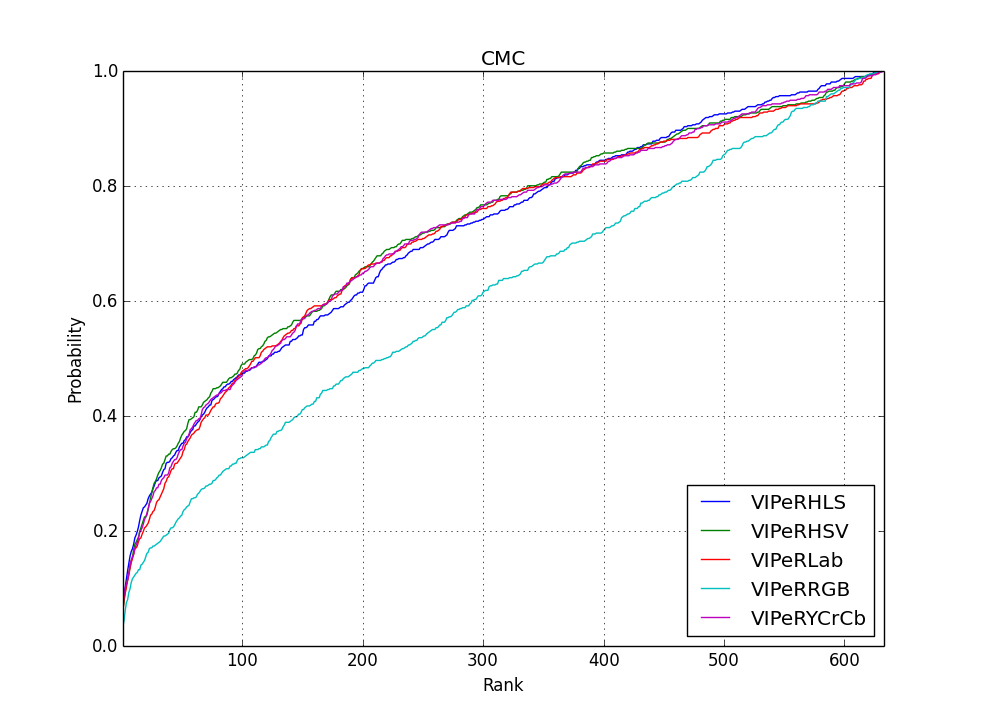
\includegraphics[width=1\linewidth]{/Users/JohnsonJohnson/Downloads/thesis_1/Figures/DifferentColorspaceCMCVIPeR.png}
\caption{A CMC comparison of color histogram on different color spaces }
\label{CMCcolorspaces}
\vspace{0em}
\end{figure} 

%-----------------------------------------------------------------------------

\textbf{Shortcoming of histogram based descriptor} The performance of histogram descriptors suffers from ignoring the spatial information. Since it doesn't consider the relative distribution of color patches. Images with same kind color patches but different distribution may have the same histogram descriptor. One example is shown in Figure \ref{RGBbgr}.

\begin{figure}[H]
\begin{minipage}[t]{0.5\linewidth}
\centering
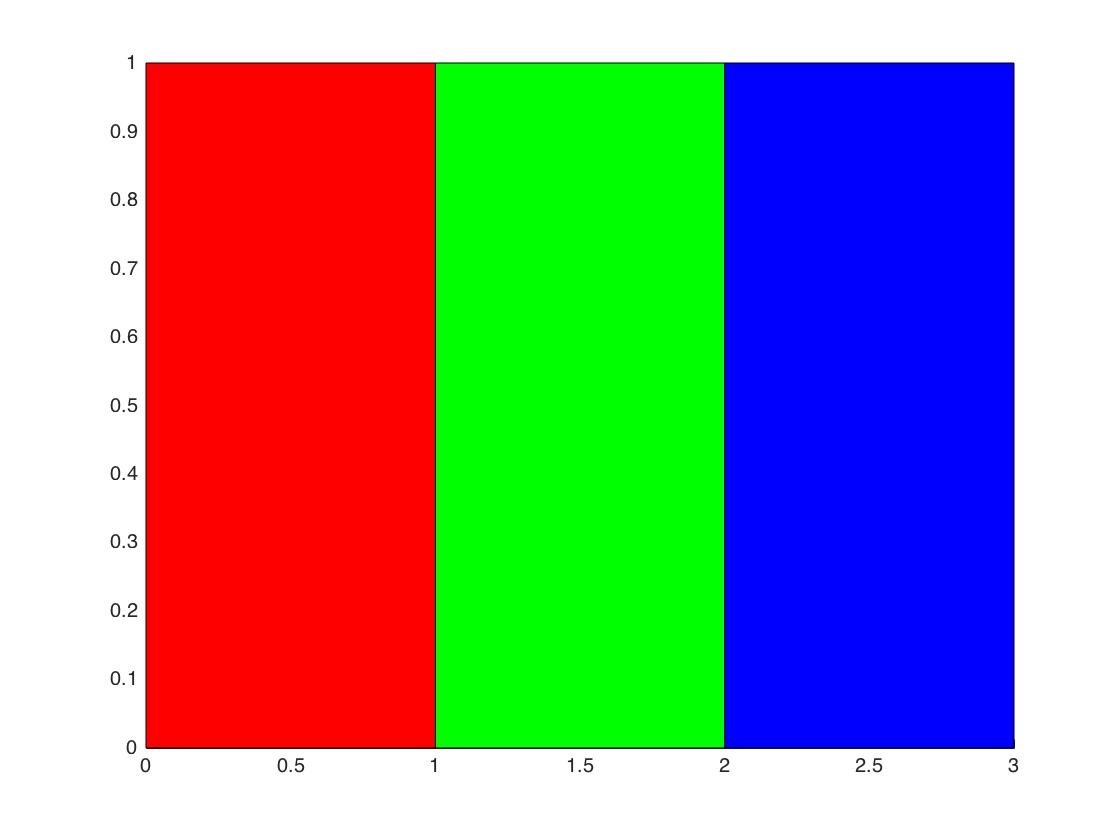
\includegraphics[width=2.2in]{/Users/JohnsonJohnson/Downloads/thesis_1/Figures/RGB.jpg}
%\caption{RGB patch}
\end{minipage}%
\begin{minipage}[t]{0.5\linewidth}
\centering
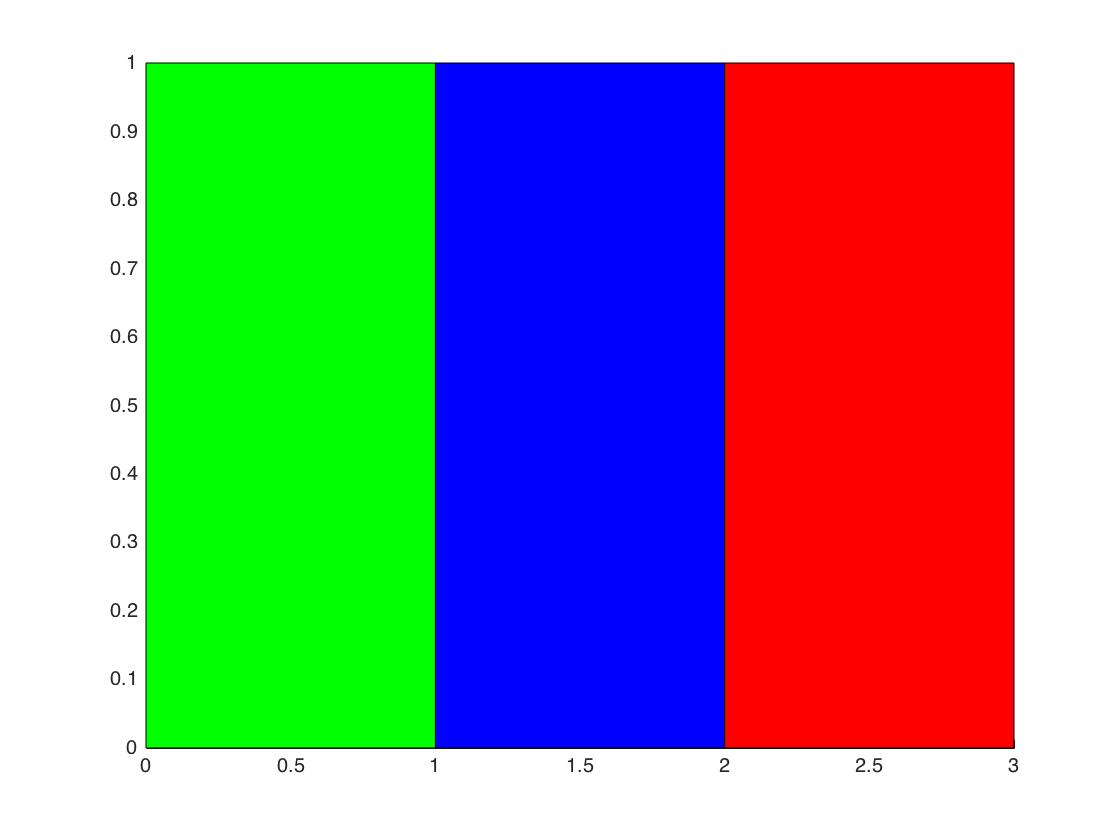
\includegraphics[width=2.2in]{/Users/JohnsonJohnson/Downloads/thesis_1/Figures/GBR.jpg}
%\caption{GBR patch}
\end{minipage}
\caption{A comparison of two patches with same entropy but different color distribution}
\label{RGBbgr}
\end{figure}


\subsection{Local binary pattern (LBP)}
Local binary pattern \cite{LBP1, LBP2} extracts the texture information with efficient computing and has been used on people detection and recognitions. Figure \ref{LBPdemoshot} is an example of LBP. by thresholding neighbour pixel of center pixel (shown in Figure \ref{LBPtheory}), the pixels are transformed into a binary integer. There are many extended LBP like tLBP, VLBP, OCLBP. Besides, LBP is well known for its robustness to monotonic illumination variation.
\begin{figure}[H]
\centering
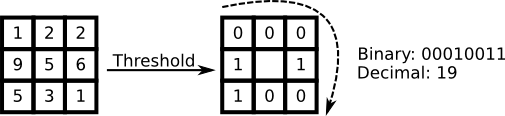
\includegraphics[width=0.8\linewidth]{/Users/JohnsonJohnson/Downloads/thesis_1/Figures/LBPdemo.png}
\caption{LBP: by thresholding the neighbour pixels the pixels are transformed into a binary number }
\label{LBPtheory}
\vspace{0em}
\end{figure}


\begin{figure}[H]
\begin{minipage}[t]{0.5\linewidth}
\centering
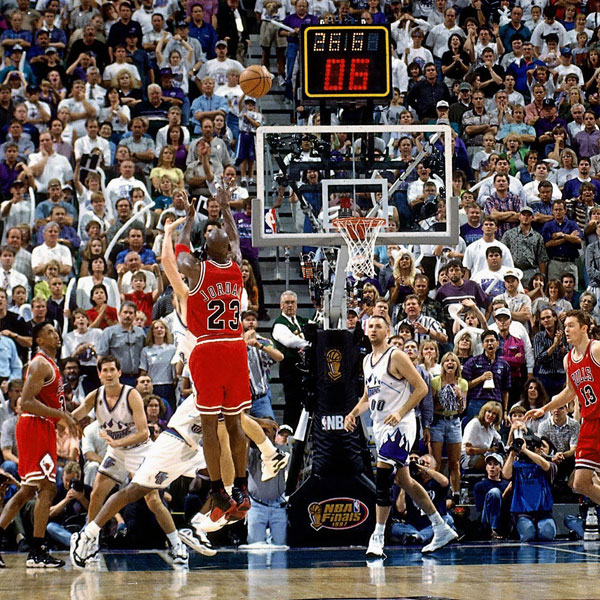
\includegraphics[width=2.2in]{/Users/JohnsonJohnson/Downloads/thesis_1/Figures/Theshot1.jpg}
\end{minipage}%
\begin{minipage}[t]{0.5\linewidth}
\centering
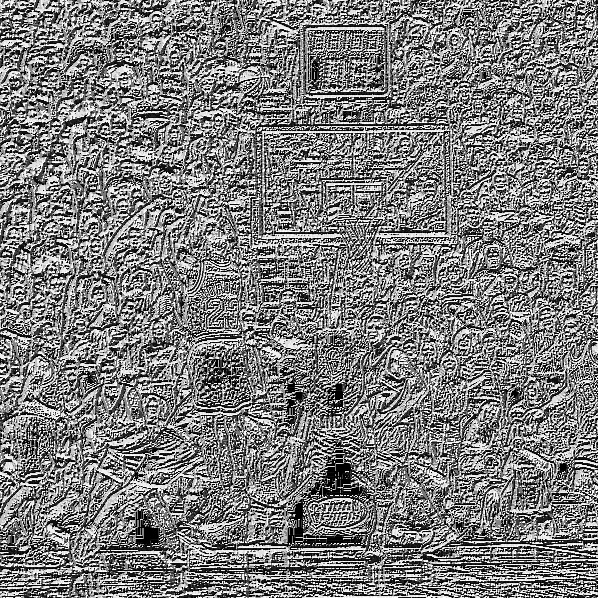
\includegraphics[width=2.2in]{/Users/JohnsonJohnson/Downloads/thesis_1/Figures/TheshotLBP1.jpg}
\end{minipage}
\caption{One LBP example}
\label{LBPdemoshot}
\end{figure}


\subsection{Histogram of oriented gradients (HOG)}
The HOG \cite{HOG} descriptor also extracts textural information of images by gradient computing. A brief introduction about its gradient computation is presented here, more details can be referenced in \cite{HOG}. In HOG feature it computes the gradient of input intensity  image $I(x, y)$ by equations 

\begin{equation}
\begin{aligned}
I_x = \frac{\partial I}{\partial x},\\
I_y = \frac{\partial I}{\partial y},
\end{aligned}
\end{equation}
the gradient can be computed fast by some discrete derivative masks below, like 1-D Sobel masks:
\begin{equation}
\begin{aligned}
Centered: M_{c} &= [-1, 0, 1]\\
Uncentered: M_{uc}& = [-1, 1]
\end{aligned}
\end{equation}
or 2-D Sobel masks:
\begin{equation}
\begin{aligned}
D_x = \left[ \begin{matrix}
0 & 1 \\
-1& 0
\end{matrix}
\right]\\
D_y = \left[ \begin{matrix}
-1 & 0 \\
0& 1
\end{matrix}
\right]
\end{aligned}
\end{equation}
or $3\times 3$ Sobel masks:
\begin{equation}
\begin{aligned}
S_x &= \left[ \begin{matrix}
-1 &0 & 1 \\
-2& 0 & 2\\
-1 &0 & 1 
\end{matrix}
\right]\\
S_y &= \left[ \begin{matrix}
1 & 2 &1 \\
0& 0 & 0\\
-1 & -2 &-1
\end{matrix}
\right]
\end{aligned}
\end{equation}

Using different masks will result different performance. Besides, gaussian smoothing is often performed before gradient computing. It has been shown that using 1-D Sobel without gaussian smoothing has the best performance. A HOG feature demo is shown in Figure \ref{fig:HOGdemo}.
\begin{figure}[H]
\centering
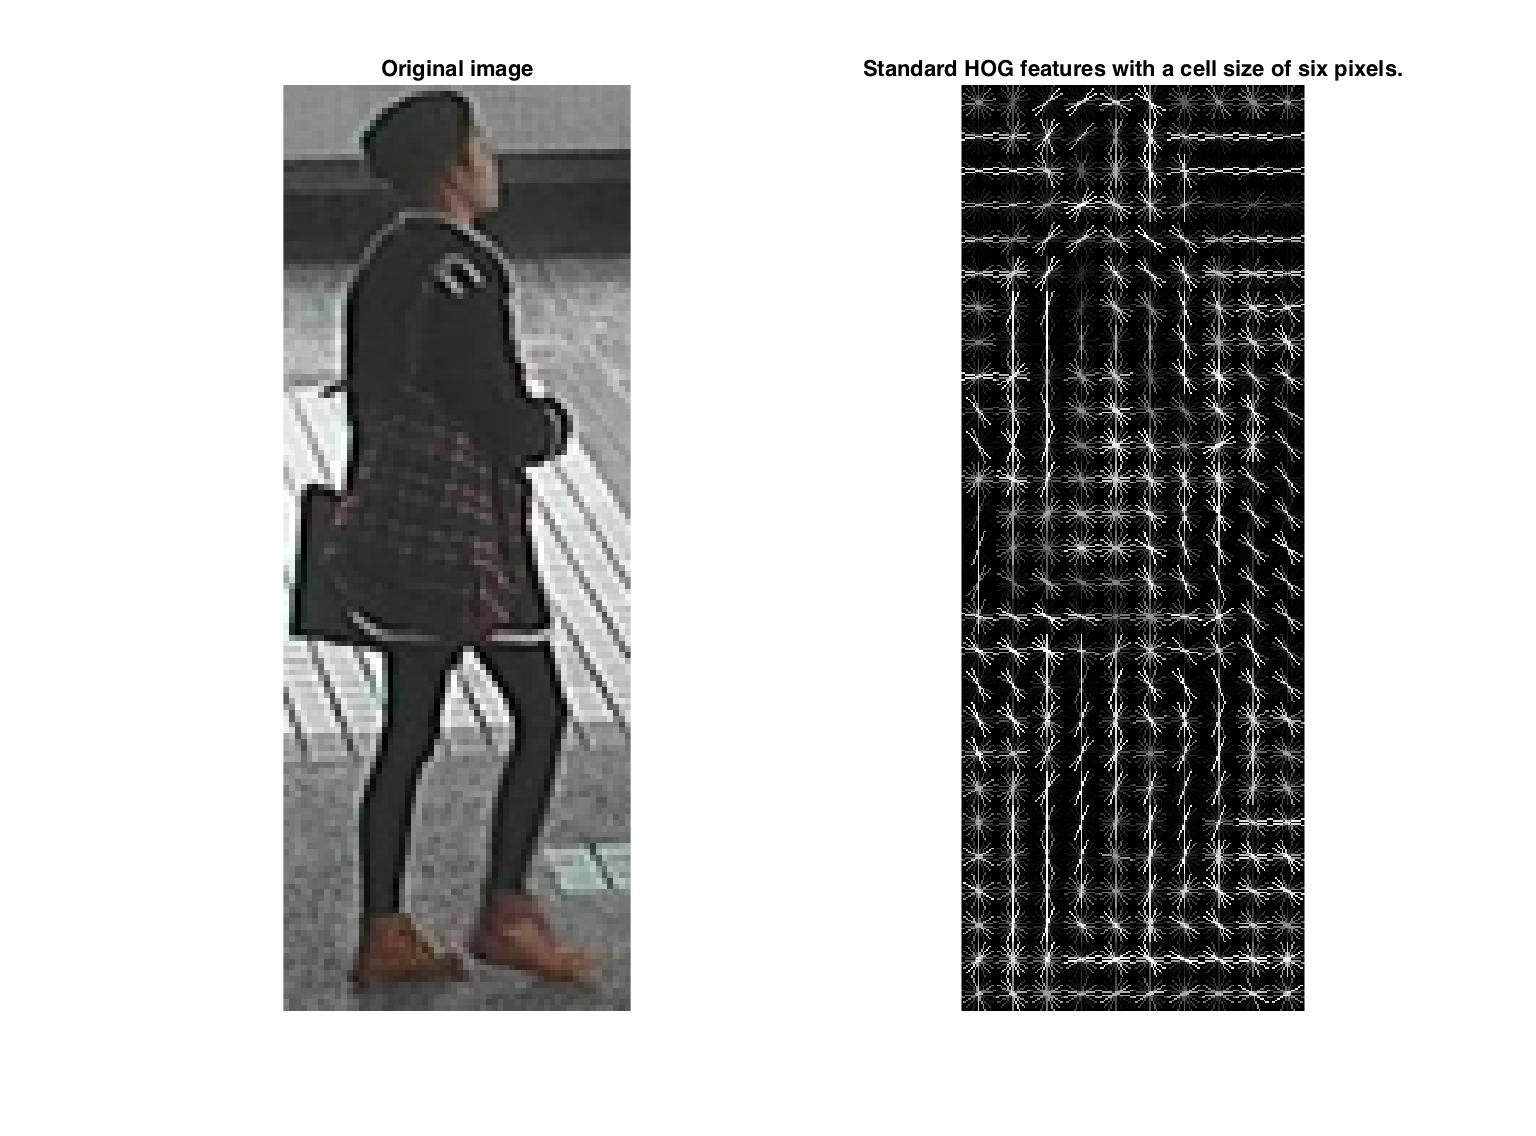
\includegraphics[width=1\linewidth]{/Users/JohnsonJohnson/Downloads/thesis_1/Figures/HOGfeatureDemo.jpg}
\caption{A demo of HOG feature with a cell size of six pixels}
\label{fig:HOGdemo} 
\vspace{0em}
\end{figure}


\section{Influence of background segmentation on different basic descriptors}
Many works try to minimize impact of background noise of pedestrians' image. It's easier to automatically segment foreground from a sequential frames or video than a single frame. In \cite{SDALF} the author provides foreground masks for all images following the algorithm in \cite{STEL}.  Some of those segmented foregrounds are shown in Figure \ref{VIPeRFGs} and it's obvious that certain body parts like head and feet are lost. To compare those loss's impact on color and textural descriptors, a comparison of foreground segmentation on HSV color histogram descriptors, LBP and HOG descriptor is given in Figure \ref{fig:SegHSV}, Figure \ref{fig:SegLBP} and Figure \ref{fig:SegHOG}. 


\begin{figure}[H]
\centering
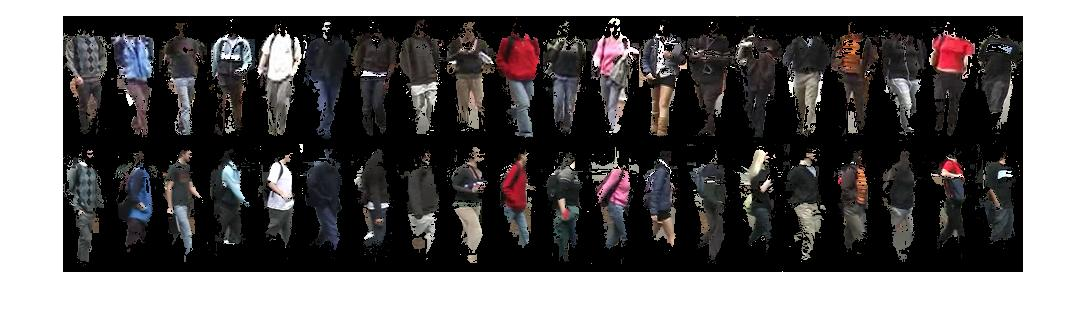
\includegraphics[width=1\linewidth]{/Users/JohnsonJohnson/Downloads/thesis_1/Figures/FGdemo2VIPeR.jpg}
\caption{Foreground segmentation of individuals from VIPeR }
\label{VIPeRFGs}
\vspace{0em}
\end{figure} 

We can find that foreground segmentation decreases LBP and HOG's performance but increases HSV color histogram's performance on VIPeR dataset greatly. The reason for this is imperfect foreground segmentation causes body parts (like head and feet) loss and mask out many parts in torso and legs. Besides, in images of some individuals a part of background scene is regarded as foreground. Since HSV color histogram doesn't handle spatial distribution but only color entropy, foreground segmentation improves its performance greatly. But since LBP and HOG handle texture for each sample patch, their performance suffer from those body parts loss and little black patches from background. What's more, we can infer that imperfect foreground segmentation will also decrease other textural feature's performance.
\begin{figure}[H]
\centering
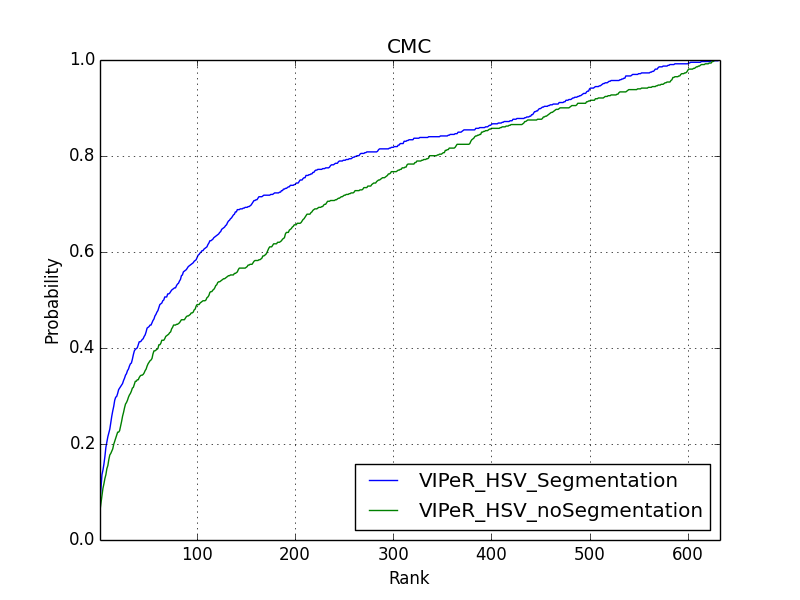
\includegraphics[width=1\linewidth]{/Users/JohnsonJohnson/Downloads/thesis_1/Figures/VIPeR_FG_HSV_comparison.png}
\caption{A CMC comparison of foreground segmentation on HSV histogram descriptor tested on VIPeR}
\label{fig:SegHSV}
\vspace{-1em}
\end{figure} 

\begin{figure}[H]
\centering
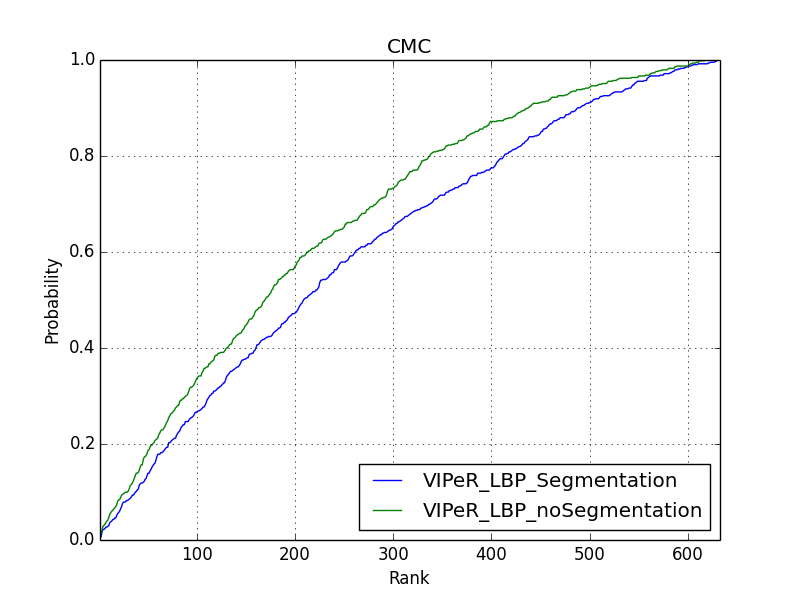
\includegraphics[width=1\linewidth]{/Users/JohnsonJohnson/Downloads/thesis_1/Figures/VIPeR_LBP_FGSegComparison.png}
\caption{A CMC comparison of foreground segmentation on LBP feature tested on VIPeR }
\label{fig:SegLBP}
\vspace{-1em}
\end{figure} 

\begin{figure}[H]
\centering
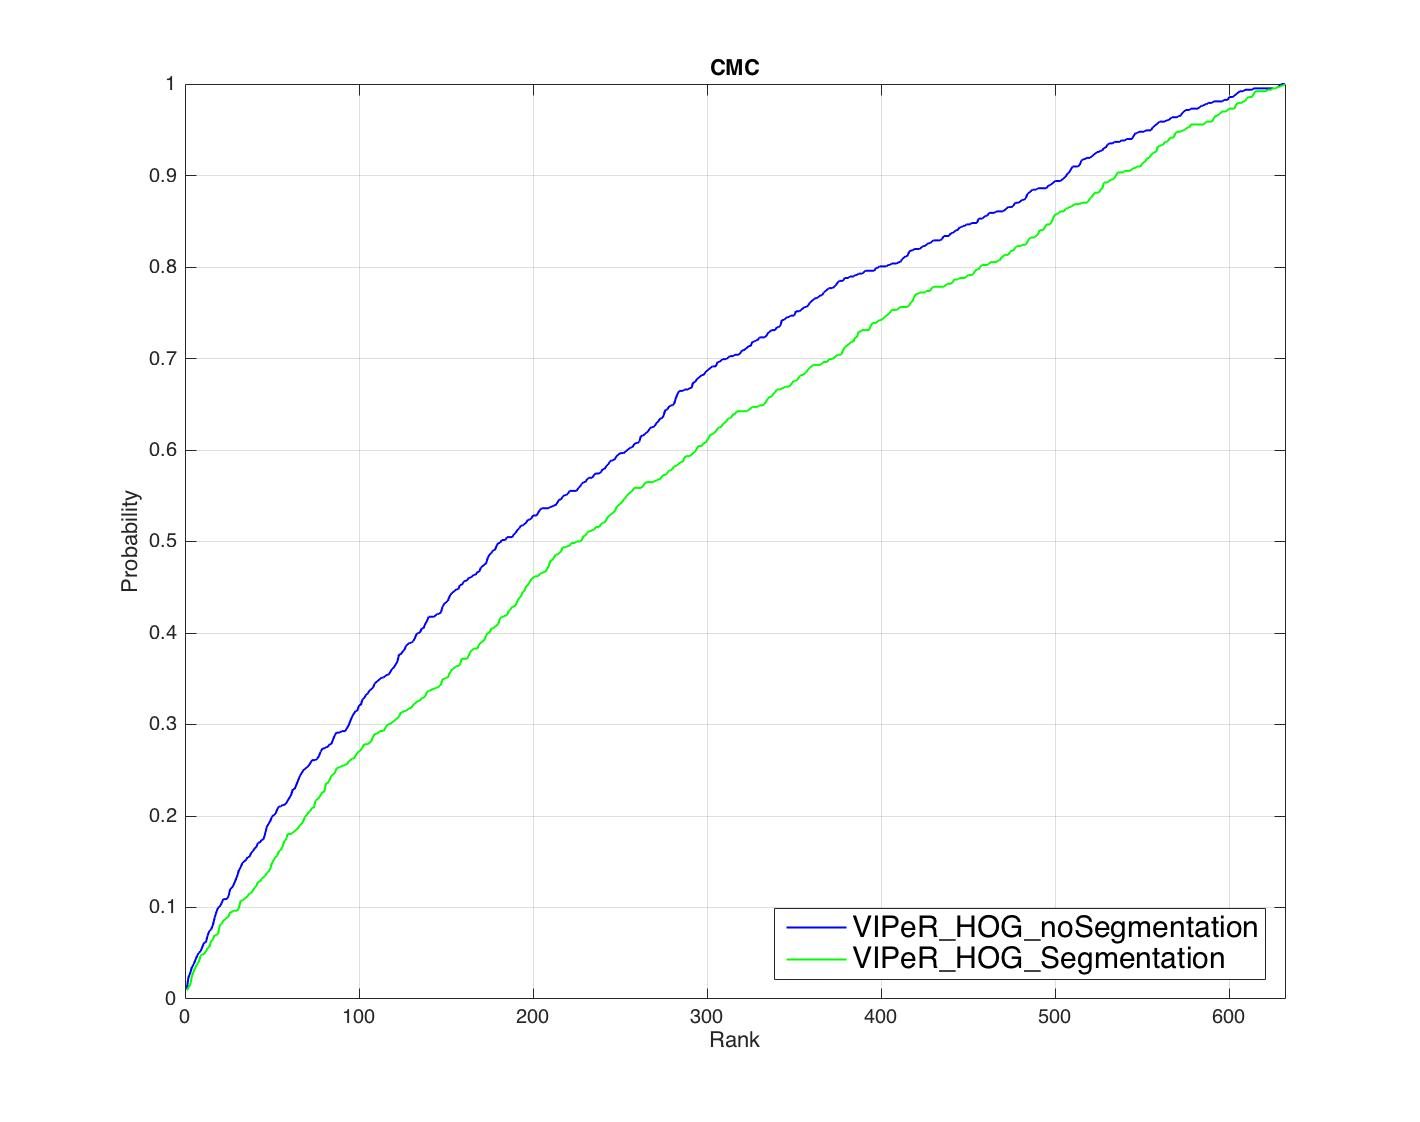
\includegraphics[width=1\linewidth]{/Users/JohnsonJohnson/Downloads/thesis_1/Figures/VIPeR_HOG_FGcomparison.jpg}
\caption{A CMC comparison of foreground segmentation on HOG feature tested on VIPeR}
\label{fig:SegHOG}
\vspace{-1em}
\end{figure} 



\section{The hierarchical gaussian descriptor}

The hierarchical gaussian descriptor is proposed by in  \cite{GOG}, this descriptor uses a two-level gaussian distribution to model an individual. This descriptor densely samples the image and models each hierarchical structure with gaussian distribution and to outperform many other works. In this thesis, all input images are sized to $128\times 64$. Firstly it divides the image into 7 overlapping horizontal slides, each slide has size $32\times 64$ and slides are overlapping by $16$ pixels vertically.  In each slide, densely sampled square patches have size of $s\times s$ pixels ($s$ = 5 in this thesis), and small patches overlaps with each other by $2$ pixels. So there is a  two-level structure in this image, small patches and slides. The small patches are first modelled with a multivariate gaussian distribution, then with those small patch gaussian distributions, the slide containing those patches is modelled with another multivariate gaussian distribution.

In a certain horizontal slide for each small patch, it's modelled by a multivariate gaussian distribution $G_p(\bm{f}_i;\bm{\mu}_p,\bm{\Sigma}_p)$, and $G_p$ can be transformed to a vector $\bm{p}$ by SPD mapping. Again, when all small patches are modelled and vectorized, the same process is repeated. Each slide is characterized by a multivariate gaussian distribution $\bm{G}_r(\bm{p};\bm{\mu}_r,\bm{\Sigma}_r)$.\\
\indent After the slide is modelled with $\bm{G}_r(\bm{p};\bm{\mu}_r,\bm{\Sigma}_r)$, the same transformation will be operated on $\bm{G}_r$ so that it's vectorized as a vector $\bm{v}$. At last all computed $\bm{v}$ are concatenated to consist of the descriptor of current image. 

\subsection{Handling the background}
In last section the impact of background subtraction on different features' performance have been studied. We've already get the result that imperfect foreground segmentation will decrease textural feature's performance. Besides, in hierarchical gaussian descriptor there is no histogram based feature computing. So in this thesis, when computing the pixel basic feature $\bm{f}_i$, the foreground segmentation is not adopted. But when modelling the region gaussian $\bm{G}_r(\bm{p};\bm{\mu}_r,\bm{\Sigma}_r)$ a weighted map is computed for each patch with equation
\begin{equation} 
N(x;\mu_0,\sigma_0) = \frac{1}{\sigma_0\sqrt{2\pi}} \exp^{\frac{(x - \mu_0)^2}{\sigma_0^2}}
\end{equation}
and here $\mu_0 = \frac{W_0}{2}, \sigma_0 = \frac{W_0}{4}$, $W_0$ is the number of patches in horizontal direction.
\subsection{Single pixel modelling}

In this hierarchical model, it is very important to have a full representation for every single pixel. To fully characterize single pixel, a $d$ dimensional vector is used to represent it. In this vector, there could be any predefined properties like coordinates, color values, texture and filter response. Suppose the original image is in RGB color space, the gaussian of gaussian descriptor uses a 8-dimensional vector $\bm{f}_i$, and 
$\bm{f}_i = (y,M_0,M_{90},M_{180},M_{270},R,G,B)$.
The y component is the y coordinate of pixel, and $M_{\{{\theta}\in{0^o,90^o,180^o,270^o}\}}$ is the quantized gradient information in 4 directions. The last three component is the color value is specified color space.

In all the benchmark dataset, all the images are cropped with a bounding box well suited the individual, and the pedestrian in an image can be at left or right of center, while in the vertical direction the head and feet of pedestrian is very close the image edge. For each pixel, the y coordinate is more correlated than x coordinate, so only y coordinate is chosen for pixel modelling. 

Then the $M$ is to characterize the texture with the gradient histogram. Different $M$ values is the magnitude of gradient in every direction. 
Firstly the gradient in x and y direction are computed by two gradient filters $\rm{h}_x$ and $\rm{h}_y$, and we have 
\begin{equation}
\begin{aligned}
h_x &= [-1, 0, 1]\\
h_y &= -h_x'
\end{aligned}
\end{equation}

Then by convolve those two filters with the intensity image $I$, the horizontal and vertical gradient $I_x, I_y$ can be computed, so the orientation and magnitude can be computed by following equations:
\begin{equation}
\begin{aligned}
O(i,j) &= (\arctan(\frac{I_y(i,j)}{I_x(i,j)}+\pi)*180 /{\pi} \\
M(i,j) &= \sqrt{(I_x(i,j)^2 + I_y(i,j))^2}
\end{aligned}
\end{equation}

The orientation are quantized into four bins by a soft voting algorithm \cite{AutoRela}. For each pixel its corresponding gradient orientation is decided by its nearest bin's direction. To make the descriptor focus on the gradient components with high values, the gradient and orientation are multiplied as follow,
\begin{equation}
M_{\theta} = MO_{\theta},
\end{equation}

%For every gradient magnitude value with its orientation , the corresponding weights of all predefined directions are computed, and the direction with the biggest weight is chosen as the quantized direction for this pixel.

To model the patch with a multi-variate gaussian distribution, we have to estimate its mean value and the covariance matrix. A multi-variate gaussian model has the form
\begin{equation}
G_p(\bm{f}_i;\bm{\mu}_p,\bm{\Sigma}_p) = \frac{\exp^{(\frac{1}{2}(\bm{f}_i-\bm{\mu}_p)^T\bm{\Sigma_p}^{-1}(\bm{f}_i-\bm{\mu}_p))}}{(2\pi)^{d/2}|{\bm{\Sigma}_p|}} 
\end{equation}
where $\bm {\mu}_p$ is the estimated mean value, and $\bm {\Sigma}_p $ is the estimated covariance matrix of current small patch. 

To estimate the parameters for this gaussian model based on sampled patches pixel features, the maximal likelihood estimate(MLE) is used. According MLE algorithm, we have the following estimated parameters
\begin{equation}
%\begin{aligned}
\bm{\mu}_p = \frac{1}{n}\sum_{i = 1}^n \bm{f}_i,
%\end{aligned}
\end{equation}
\begin{equation}
%\begin{aligned}
\bm{\Sigma}_p = \frac{1}{n-1} \sum_{i = 1}^n(\bm{f}_i-\bm{\mu})(\bm{f}_i-\bm{\mu})^T,
%\end{aligned}
\end{equation}

where $n$ is the number of pixels in current patch. When the gaussian model is computed, the next step is to model all the patch gaussians. But it's a complex problem to directly model those multivariate gaussian functions. So some transformation will be operated on estimated parameters $\bm{\mu}_p$ and $\bm{\Sigma}_p$.


%% --------------------------------------Riemannian manifold based SPD transformation
\subsection{Riemannian manifold based SPD transformation}

As described before this hierarchical gaussian descriptor is a stochastic feature, so operations like computing mean and covariance need to be operated on previous summarized gaussian distributions. Mean and covariance operation in Euclidean space can not be directly finished on previous estimated gaussian functions. A transformation is needed to make stochastic summarization feasible on patch gaussian function.
In fact, the multivariate gaussian model is a Riemannian manifold and can be embedded into a semi-positive definite matrix (SPD) space. The gaussian function is mapped into a vector space by Equation \ref{SPDmapping}. A $d$ dimensional multivariate gaussian function can be mapped into a $d+1$ dimensional $SPD_+$ space. According to \cite{MultiVarGau}, the mapping can be denoted as 
\begin{equation}\label{SPDmapping}
G(\bm{x}_i;\bm{\mu}_i,\bm{\Sigma}_i) \sim \bm{P}_i  = |\bm{\Sigma}_i|^{1/(d+1)} \left[ \begin{matrix}
\bm{\Sigma}_i + \bm{\mu}_i\bm{\mu}^T & \bm{\mu}_i \\
\bm{\mu}_i^T & 1
\end{matrix}
\right]
\end{equation}
The covariance matrix $\bm{\Sigma}_i$ can be singular for small number of pixels within the patch, to avoid this problem a regular factor $\lambda$ is added to $\bm{\Sigma}_i$ so that $\bm{\Sigma}_i = \bm{\Sigma}_i + \lambda\bm{I}$. 

After this mapping, the $n+1$ dimensional SPD matrix needs to be transformed into a vector. The matrix logarithm is used to transform it to tangent space. A $d+1$ dimensional SPD matrix can be mapped as a $d*(d+3)/2+1$ vector, which can be denoted as $SPD_i^+ \sim \bm{p}_i = vec(log(\bm{P}_i))$. Since $\bm{P}_i$ is a positive symmetric matrix, it can be compressed by half that only the upper triangular elements are preserved. To ensure its norm-1 remain the same after compression, the magnitude of off-diagonal elements in $\bm{P}_i$ are timed by $\sqrt2$.  Let $\bm{Q}=\log{\bm{P}_i}$, we have
\begin{equation}\label{vectorize}
%\begin{aligned}
 \bm{p}_i = [\bm{Q}_{1,1},\sqrt2\bm{Q}_{1,2},\sqrt2\bm{Q}_{1,3},\cdots,\sqrt2\bm{Q}_{1,d+1},
 \end{equation}
 \begin{equation}
 \bm{Q}_{2,2},\sqrt2\bm{Q}_{2,3,},\cdots,\sqrt2\bm{Q}_{2,d+1,},\cdots,\bm{Q}_{d+1,d+1,}]
%\end{aligned}
\end{equation}


Again we model the slide with a multivariate gaussian distribution $\bm{G}_r$ by equation
\begin{equation}
G_p(\bm{p}_j;\bm{\mu}_r,\bm{\Sigma}_r) = \frac{\exp^{(\frac{1}{2}(\bm{p}_j-\bm{\mu}_r)^T\bm{\Sigma_r}^{-1}(\bm{p}_j-\bm{\mu}_r))}}{(2\pi)^{d/2}|{\bm{\Sigma}_r|}} 
\end{equation}
we have known that all patches inside this slide been represented as vector $\bm{p}_j$, thus the mean $\bm{\mu}_r$ and covariance matrix ${\bm{\Sigma}}_r$ of $\bm{G}_r$ can be computed by MLE with equations
\begin{equation}
%\begin{aligned}
\bm{\mu}_r = \frac{1}{m}\sum_{j = 1}^m \bm{p}_j,
%\end{aligned}
\end{equation}
\begin{equation}
%\begin{aligned}
\bm{\Sigma}_r = \frac{1}{m -1} \sum_{j = 1}^m(\bm{p}_j-\bm{\mu}_r)(\bm{p}_j-\bm{\mu}_r)^T,
%\end{aligned}
\end{equation}
m is the total number pf patches inside current slide. Again $\bm{\mu}_r$ and $\bm{\Sigma}_r$ are mapped to a SPD space by equation
\begin{equation}
G(\bm{p};\bm{\mu}_r,\bm{\Sigma}_r) \sim \bm{P}_r  = |\bm{\Sigma}_r|^{1/(d+1)} \left[ \begin{matrix}
\bm{\Sigma}_r + \bm{\mu}_r\bm{\mu}_r^T & \bm{\mu}_r \\
\bm{\mu}_r^T & 1
\end{matrix}
\right]
\end{equation}
and $\bm{P}_r$ is vectorized by Equation \ref{vectorize}.

When all horizontal slides' descriptor computed they are concatenated to form the descriptor for the whole image.



%%Integral image for fast computing
\subsection{Integral image for fast region covariance computation}

To compute estimated parameters for all those overlapping small patches, the time complexity of computing one by one patch is gigantic because there are many repeating computations. To compute the estimated covariance matrix \bm{$\Sigma}$ for every small patch with size of $W\times H$, the integral image is used to reduce time complexity. The integral image \cite{RegionCovariance} is a intermediate representation to fast compute rectangle area sum in an image. Each pixel value in integral image is the sum of all the pixels inside the rectangle bounded by current pixel and the upper left pixel. That is, the integral image S(x, y) for image I(x, y) is 
\begin{equation}
S(x', y') = \sum_{x<x', y <y'} I(x, y),
\end{equation}

\begin{figure}[H]
\centering
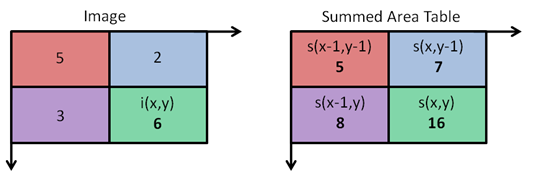
\includegraphics[width=1\linewidth]{/Users/JohnsonJohnson/Downloads/thesis_1/Figures/IntegralImage.png}
\caption{Integral image}
\vspace{0em}
\end{figure} 
By using integral image any rectangular region sum can be computed in constant time. \\
\indent To compute the covariance matrix of a certain rectangle area in a $W\times H\times d$ dimensional feature tensor $F$, suppose $\bm{I}_F$ is the $W\times H\times d$ tensor of integral images of $F$, we have 
\begin{equation}
 \bm{I}_F(x', y', i) = \sum_{x < x', y < y'}F(x, y ,i), i = 1 \dots d
\end{equation} 
and suppose the $\bm{C}(x', y', i, j)$ is the $W\times H\times d\times d$ tensor of second order integral images, we have
\begin{equation}
\bm{C}(x', y', i, j) = \sum_{x<x', y<y'} F(x, y, i)F(x, y, j), i, j = 1 \dots d.
\end{equation}
let $\bm{I}_{x, y}$ be the $d$ dimensional vector in $\bm{I}_F$, $\bm{C}(x, y)$ be the $d\times d$ dimensional matrix in $\bm{C}$, 
\begin{equation}
\begin{aligned}
\bm{I}_{x, y} = [ \bm{I}_F(x', y', 1) \dots  \bm{I}_F(x', y', d)]^T \\
 \bm{C}_{x, y} = \left [
 \begin{matrix} 
 \bm{C}(x, y, i, 1)  &\cdots & \bm{C}(x, y, 1, d)\\
 			     & \ddots &			        \\
\bm{C}(x, y, d, 1)   & \cdots &\bm{C}(x, y, d, d)
 
 \end{matrix} \right ]
 \end{aligned}
\end{equation}

Then for any rectangule regions $R(x', y'; x'', y'')$, where $(x', y')$ is the upper left coordinate and $(x'', y'')$ is the lower right coordinate, the covariance matrix can be compute as 
\begin{equation}
\begin{aligned}
\bm{C}_R(x', y'; x'', y'') = \frac{1}{n-1} [\bm{C}_{x'', y''} + \bm{C}_{x', y'} -  \bm{C}_{x'', y'}-  \bm{C}_{x', y''} \\
-\frac{1}{n}(\bm{I}_{x'', y''} + \bm{I}_{x'', y''} - \bm{I}_{x', y''} - \bm{I}_{x'', y'})(\bm{I}_{x'', y''} + \bm{I}_{x'', y''} - \bm{I}_{x', y''} - \bm{I}_{x'', y'})^T]
\end{aligned}
\end{equation}
where $n$ is the number of feature vector in $F$, and $n = (x'' - x')(y'' - y')$. By creating the integral image the covariance of any rectangular area in $F$ can be computed in $O(d^2)$ time.

When all patches in a region are computed, the same process is repeated to compute the region gaussian. 



\textbf{Dimension analysis} It has been known that combination of descriptors of different color space can greatly improve re-ID performance. In this project, the hierarchical gaussian descriptor in RGB color space is the base descriptor. Descriptors in three more color space \{HSV, Lab, nRGB\} are extracted. The nRGB color space is calculated as 
\begin{equation}
\begin{aligned}
nR = \frac{R}{R+G+B},\\
nG = \frac{G}{R+G+B},\\
nR = \frac{B}{R+G+B}, 
\end{aligned}
\end{equation}

since $nB$ can be calculated with $nR$ and $nG$, in this color space only the first two channel values are used to reduce redundancy. Therefore, for color space \{RGB, HSV, Lab, nRGB\}, the corresponding dimension of pixel feature is \{8, 8, 8, 7\}. After the matrix to vector transformation, the dimension of patch gaussian vector of each channel is \{45, 45, 45, 36\}. Again after the patch gaussian to region gaussian transformation, the dimension of each channel is \{1081, 1081, 1081, 703\}. Suppose there are 7 horizontal slides in each image, the dimension of concatenated descriptor of each channel is \{7567, 7567, 7567, 4921\}. If four color space are all used, the dimension is the sum of each channel as 27622. 


%\section{Kernel fisher discriminant analysis}
%The extracted hierarchical gaussian descriptors have high dimension, it's intractable to learn a SPD matrix with such a high dimension. Dimension reduction is required to learn a subspace.
%Among those methods to reduce dimension, principal component analysis (PCA) is often used. However, PCA is an unsupervised dimension reduction and may have a low performance for those reasons, $(1)$, PCA is to maximize the variance of dimension reduced data, and as a unsupervised method it doesn't has a full consideration of the the relation of between and within classes, it is very likely that the descriptors of different classes can be mixed up after the dimension reduction; $(2)$ PCA may suffer from the small sample size problem. In some Re-ID datasets, there may be two or less images for each pedestrian in each viewpoint (like VIPeR), if the dimension of descriptor is much bigger than sample size, much information can be lost with PCA. In this thesis, the kernel local fisher discriminant analysis (KLFDA) is used to reduce dimension. 
%\subsection{Fisher discriminant analysis (FDA)}
%KLFDA is the kernel version of LFDA, and LFDA is a combination of Fisher discriminant analysis[ ] and and the locality preserving projection in [LPP ] and kernel method. A brief introduction of FDA, LPP and kernel method is introduced below.
%
%FDA is a supervised dimension reduction and its input contains the class labels. For a set of $d$-dimensional observations $\bm{x}_i$, where $i\in\{1,2,\cdots,n\}$, the label $l_i\in\{1,2,\cdots,l\}$. Two matrix are defined as the intraclass scatter matrix $\bm{S}^{(w)}$ and between class scatter matrix
%$\bm{S}^{(b)}$, 
%\begin{equation}
%\begin{aligned}
%\bm{S}^{(w)} &= \mathop{\sum} _{i=1}^l\mathop{\sum}_{j:l_j = i} (\bm{x}_j - \bm{\mu}_i)(\bm{x}_j - \bm{\mu}_i)^T \\
%\bm{S}^{(b)}  &= \mathop{\sum} _{i=1}^l n_i(\bm{\mu}_i - \bm{\mu})(\bm{\mu}_i - \bm{\mu})^T
%\end{aligned}
%\end{equation}
%where the $\bm{\mu}_i$ is the mean of samples whose label is $i$, and $\bm{\mu}$ is the mean of all samples,
%\begin{equation}
%\begin{aligned}
%\bm{\mu}_i &= \frac{1}{n_i} \sum \bm{x}_i, \\
%\bm{\mu} &= \frac{1}{n} \sum \bm{x}_i
%\end{aligned}
%\end{equation}
%
%The Fisher Discriminant Analysis transform matrix $\bm{T}$ can be represented as 
%\begin{equation}
%\bm{T} = \arg\max \frac{\bm{T}^T\bm{S}^{(b)}\bm{T}}{\bm{T}^T\bm{S}^{(w)}\bm{T}}
%\end{equation}
%This equation can be solved by Lagrange multiplier method, we define a Lagrange function 
%\begin{equation}
%L(\bm{t}) = \bm{t}^T\bm{S}^{(b)}\bm{t} - \lambda(\bm{t}^T\bm{S}^{(w)}\bm{t} - 1)
%\end{equation}
%Then the differential respect to $\bm{t}$ is 
%\begin{equation}
%\frac{\partial L(\bm{t})}{\partial \bm{t}} = 2\bm{S}^{(b)}\bm{t} - 2\lambda \bm{S}^{(w)}\bm{t}
%\end{equation}
%
%let 
%\begin{equation}
%\frac{\partial L(\bm{t})}{\partial \bm{t}} = 0
%\end{equation}
%
%we can get 
%\begin{equation}
%\bm{S}^{(b)}\bm{t}_i  = \lambda \bm{S}^{(w)}\bm{t}_i
%\end{equation}
%\label{eigen1}
%
%here $\bm{t}_i$ is the $i_{th}$ column of $\bm{T}$, and the optimization problem is converted to a eigenvalue decomposition problem. 
%
%Fisher discriminant analysis tries to minimize the intraclass scatter matrix while maximize the interclass scatter matrix, and $\bm{T}$ is computed by the eigenvalue decomposition. $\bm{T}$ can be represented as the set of all the corresponding eigenvectors, as $ \bm{T} = (\bm{t}_1,\bm{t}_2,\cdots,\bm{t}_k)$.
%
%FDA has a form similar with signal and noise ratio, however, the FDA dimension reduction may have poor performance for it doesn't consider the locality of data. An example of this is the multimodality[]. Multimodality is the case many clusters are formed in the same class. 
%\subsection{Locality preserving projection (LPP)}
%
%In \cite{LPP} locality preserving projection (LPP) is proposed to exploit data locality. An affinity matrix is created to record the affinity of sample $\bm{x}_i$ and $\bm{x}_j$,  typically the range of elements in $\bm{A}_{i,j}$ is $[0,1]$. There are many manners to define a $n \times n$ affinity matrix $\bm{A}$, usually two sample points with a smaller distance has a higher affinity value than those with bigger distance value. One of them is if  $\bm{x}_i$ is within k-nearest neighbours of $\bm{x}_j$ then $\bm{A}_{i,j} = 1$ otherwise  $\bm{A}_{i,j} = 0$.  
%
%Another diagonal matrix $D$ can be defined that each diagonal element is the sum of corresponding column in $\bm{A}$,
%\begin{equation}
%\bm{D}_{i,i} = \mathop{\sum}_{j=1}^n \bm{A}_{i, j} 
%\end{equation}
%then the LPP transform matrix is defined as follow,
%\begin{equation}
%\bm{T}_{LPP} = \mathop{\arg\min}_{\bm{T}\in\bm{R}^{d\times m}} \frac{1}{2}\mathop{\sum}_{i, j= 1}^n \bm{A}_{i,j} ||\bm{T}^T\bm{x}_i - \bm{T}^T\bm{x}_j||
%\end{equation}
%so that $ \bm{T}^T\bm{X}\bm{D}\bm{X}^T\bm{T} = \bm{I} $.
%Suppose the subspace has a dimension of $m$, then LPP transform matrix $T$ can be represented as 
%
%$$\bm{T}_{LPP} = \{ \bm{\phi}_{d-m+1} | \bm{\phi}_{d-m+2} | \cdots \bm{\phi}_{d}\} $$
%
%And each $\bm{\phi}$ in $T$ is the eigenvector of following fomula,
% \begin{equation}
%\bm{X}\bm{L}\bm{X}^T\bm{\phi} = \gamma\bm{X}\bm{D}\bm{X}^T
%\end{equation}
%where $\gamma$ is corresponding eigenvalue of $\bm{\phi}$, and $L = D - A$.\\
%%But the LPP dimension reduction is still not discriminant enough, 
%\subsection{Local fisher discriminant analysis}
%\indent LFDA \cite{LFDA} combines FDA and LPP and have better performance. The key in LFDA is it assigns weights to elements in $\bm{A}^{(w)}$ and $\bm{A}^{(b)}$, so that,
%\begin{equation}
%\begin{aligned}
%\bm{S}^{(w)} &= \frac{1}{2}\sum _{i=1}^l\sum_{j:l_j = i} \bm{A}_{i,j}^w (\bm{x}_j - \bm{\mu}_i)(\bm{x}_j - \bm{\mu}_i)^T \\
%\bm{S}^{(b)} &=  \frac{1}{2}\sum _{i=1}^l \bm{A}_{i,j}^b(\bm{\mu}_i - \bm{\mu})(\bm{\mu}_i - \bm{\mu})^T
%\end{aligned}
%\end{equation}
%where 
%
%\begin{equation}
%\begin{aligned}
%\bm{A}_{i,j}^{(w)} = \left \{ 
%\begin{array}{rcl}
%\bm{A}_{i,j}/n_c &  &y_i = y_j \\
%0 & & else
%\end{array}
%  \right.  \\
%  \bm{A}_{i,j}^{(b)} = \left \{ 
%\begin{array}{rcl}
%(\frac{1}{n} - \frac{1}{n_c})  \bm{A}_{i,j} &  &{y_i = y_j }\\
%\frac{1}{n} & & {else}
%\end{array}
%  \right. 
% \end{aligned}
%\end{equation}
%where $y_i$ is the class label of sample point $\bm{x}_i$. So the transformation matrix $T_LFDA$ can be computed by equation
%\begin{equation}
%\bm{T}_{LFDA}  = \arg\min_{\bm{T}} (\frac{\bm{T}^T\bm{S}^{(b)}\bm{T}}{\bm{T}^T\bm{S}^{(w)}\bm{T}})
%\end{equation}
%\label{eigencompute1} 
%Again this problem can be solved by eigenvalue decomposition by equation \ref{eigen1}. 
%
%
%
%When applying the LFDA to original high dimensional descriptors, one problem is the computation cost. Suppose the vector data has a dimension of $d$, LFDA has to solve the eigenvalue a matrix with dimension $d\times d$. In some descriptors the $d$ could be more than 20000 and thus the computation cost is intractable. 
% 
%\subsection{Kernel local fisher discriminant analysis(KLFDA)}
%
%KLFDA  \cite{KLFDA} is the nonlinear version of LFDA. Most dimensionality reduction methods including PCA, LDA and LFDA are linear dimensionality reduction methods. However, when descriptors data are non-linear in feature space, its hard to capture its between-class discriminant information with linear reduction methods. One alternative method is to nonlinearly map input descriptors $\bm{x}_i$ to higher dimensional feature space $\Phi$ by a function $\phi(\bm{x}_i)$, again the LFDA is performed in feature space $\Phi$. Thus the transformation matrix $T$ can be computed by equation
%\begin{equation}
%\bm{T} = \arg \min \frac{\bm{T}^T\bm{S}^{(b)}_{\phi}\bm{T}}{\bm{T}^T\bm{S}^{(w)}_{\phi}\bm{T}}
%\end{equation}
%where $\bm{S}^{(b)}_{\phi}$ and $\bm{S}^{(w)}_{\phi}$ is the between class scatter and within class scatter in mapped feature space $\Phi$.
%
%Note that the transformation matrix $\bm{T} \in \Phi$, it's computationally expensive to explicitly compute the mapping function $\phi$ and perform LFDA in feature space $\Phi$ because the dimension of $\Phi$ may be infinite. Rather than explicitly computing, the mapping function $\phi$ can be implicit and the feature space $\Phi$ can be defined by the inner product of features in $\Phi$. Kernel trick [] is used here and a kernel function can be defined as the inner product of mapped vectors $\phi(\bm{x}_i)$ and $\phi(\bm{x}_j)$ by equation
% \begin{equation}
% k(\bm{x}_i,\bm{x}_j) = <\phi(\bm{x}_i),\phi(\bm{x}_j)>,
% \end{equation}
% the $< \cdot >$ is the inner product. There are many kinds of kernel like linear kernel, polynomial kernel and radial basis function (RBF) kernel. In this paper the RBF kernel is adopted. A RBF kernel is defined as 
% \begin{equation}
% k_{RBF}(\bm{x}_i,\bm{x}_j) = \exp^{(-\gamma||\bm{x}_i-\bm{x}_j||^2)}. 
% \end{equation}
%Suppose $\bm{X}$ is the sample descriptors matrix, and we have
%\begin{equation}
%\bm{X} = (\bm{x}_1, \bm{x}_2,\cdots, \bm{x}_n), 
%\end{equation}
%and the label vector is $\bm{l} = (l_1, l_2, \cdots, l_n)$. Then the kernel matrix of $\bm{X}$ can be computed as following equation:
%\begin{equation}
%\bm{K} =  \phi(\bm{X})^T \phi(\bm{X})
%\end{equation}
%and we have 
%\begin{equation}
%\bm{K}_{i,j} =  k(\bm{x}_i,\bm{x}_j) = <\phi(\bm{x}_i),\phi(\bm{x}_j)> =  \exp^{(-\gamma||\bm{x}_i-\bm{x}_j||^2)}
%\end{equation}
%
%In \cite{LFDAdr} the authors proposed fast computation of LFDA by replacing $\bm{S}^{(b)}$ with the local scatter mixture matrix $\bm{S}^{(m)}$defined by 
%\begin{equation}
%\begin{aligned}
%\bm{S}^{(m)} &= \bm{S}^{(b)} + \bm{S}^{(w)}\\
%\bm{S}^{(m)} &= \frac{1}{2} \sum_{i,j = 1} \bm{A}_{i,j}^{(m)} (\bm{x}_i - (\bm{x}_j)(\bm{x}_i - (\bm{x}_j)^T
%\end{aligned}
%\end{equation}
%and 
%
%\begin{equation}
%\bm{A}_{i,j}^{(m)} = \bm{A}_{i,j}^{(w)}  + \bm{A}_{i,j}^{(w)}
%\end{equation}
%
%\noindent according to indentify(Fukunaga, 1990)
%\begin{equation}
%tr((\bm{T}^T\bm{S}^{(w)}\bm{T})^{(-1)}(\bm{T}^T\bm{S}^{(m)}\bm{T}) = tr((\bm{T}^T\bm{S}^{(w)}\bm{T})^{(-1)}(\bm{T}^T\bm{S}^{(b)}\bm{T}) + m
%\end{equation}
%equation \ref{eigencompute1} is equal to 
%
%\begin{equation}
%\bm{T}_{LFDA}  = \arg\min_{\bm{T}} (\frac{\bm{T}^T\bm{S}^{(m)}\bm{T}}{\bm{T}^T\bm{S}^{(w)}\bm{T}})
%\end{equation}
%and it can be transformed into a eigenvalue decomposition problem 
%\begin{equation}
%\bm{S}^{(m)}\bm{t}_i  = \lambda \bm{S}^{(w)}\bm{t}_i
%\end{equation}
%\label{eigen2}
%Also with the replacement of $\bm{S}^{(m)}$, in \cite{LFDAdr} the author summarized that 
%\begin{equation}
%\bm{S}^{(m)} = \bm{X}\bm{L}^{(m)}\bm{X}^T
%\end{equation}
%where $\bm{L}^{(m)}  = \bm{D}^{(m)} - \bm{A}^{(m)}$, and $ \bm{D}^{i,i} = \sum_{j=1}^n  \bm{A}^{(m)}$. Also $\bm{S}^{(w)}$ can be represented as 
%\begin{equation}
%\bm{S}^{(w)} = \bm{X}\bm{L}^{(w)}\bm{X}^T
%\end{equation}
%where $\bm{L}^{(w)}  = \bm{D}^{(w)} - \bm{A}^{(m)}$, and $ \bm{D}^{i,i} = \sum_{j=1}^n  \bm{A}^{(w)}$. 
%Therefore, equation \ref{eigen2} can be represented as
%\begin{equation}
%\bm{X}\bm{L}^{(m)}\bm{X}^T \bm{t}_i= \lambda\bm{X}\bm{L}^{(w)}\bm{X}^T \bm{t}_i
%\end{equation}
%\label{equationS}
%the eigen vector $\bm{t}_i$  can be represented as $\bm{t}_i = \bm{X}\gamma, vector \gamma_i \in R^n$, with this replacement, we left multiply $\bm{X}^T$ to equation \ref{equationS} to get 
%\begin{equation}
%\bm{X}^T\bm{X}\bm{L}^{(m)}\bm{X}^T\bm{X}\gamma_i = \lambda\bm{X}^T\bm{X}\bm{L}^{(w)}\bm{X}^T \bm{X}\gamma_i
%\end{equation}
%and by the kernel trick, its represented as
%\begin{equation}
%\bm{K}\bm{L}^{(m)}\bm{K}\gamma_i  = \lambda \bm{K}\bm{L}^{(w)}\bm{K}\gamma_i
%\end{equation}
%One example of using KLFDA to reduce dimension and classify the nonlinear data clusters can be shown in figure \ref{KLFDAdemo1}, \ref{KLFDAdemo2} and \ref{KLFDAdemo3}. Three classes with five clusters are distributed on a 2-D plane, by KLFDA dimension reduction its 1-D dimension reduced data distribution are shown in figure \ref{KLFDAdemo2} and figure \ref{KLFDAdemo3}. It shows that for those clusters the gaussian kernel are better than linear kernel because the dimensional reduced data are more separate when using gaussian kernel function.
%
%\begin{figure}[H]
%\centering
%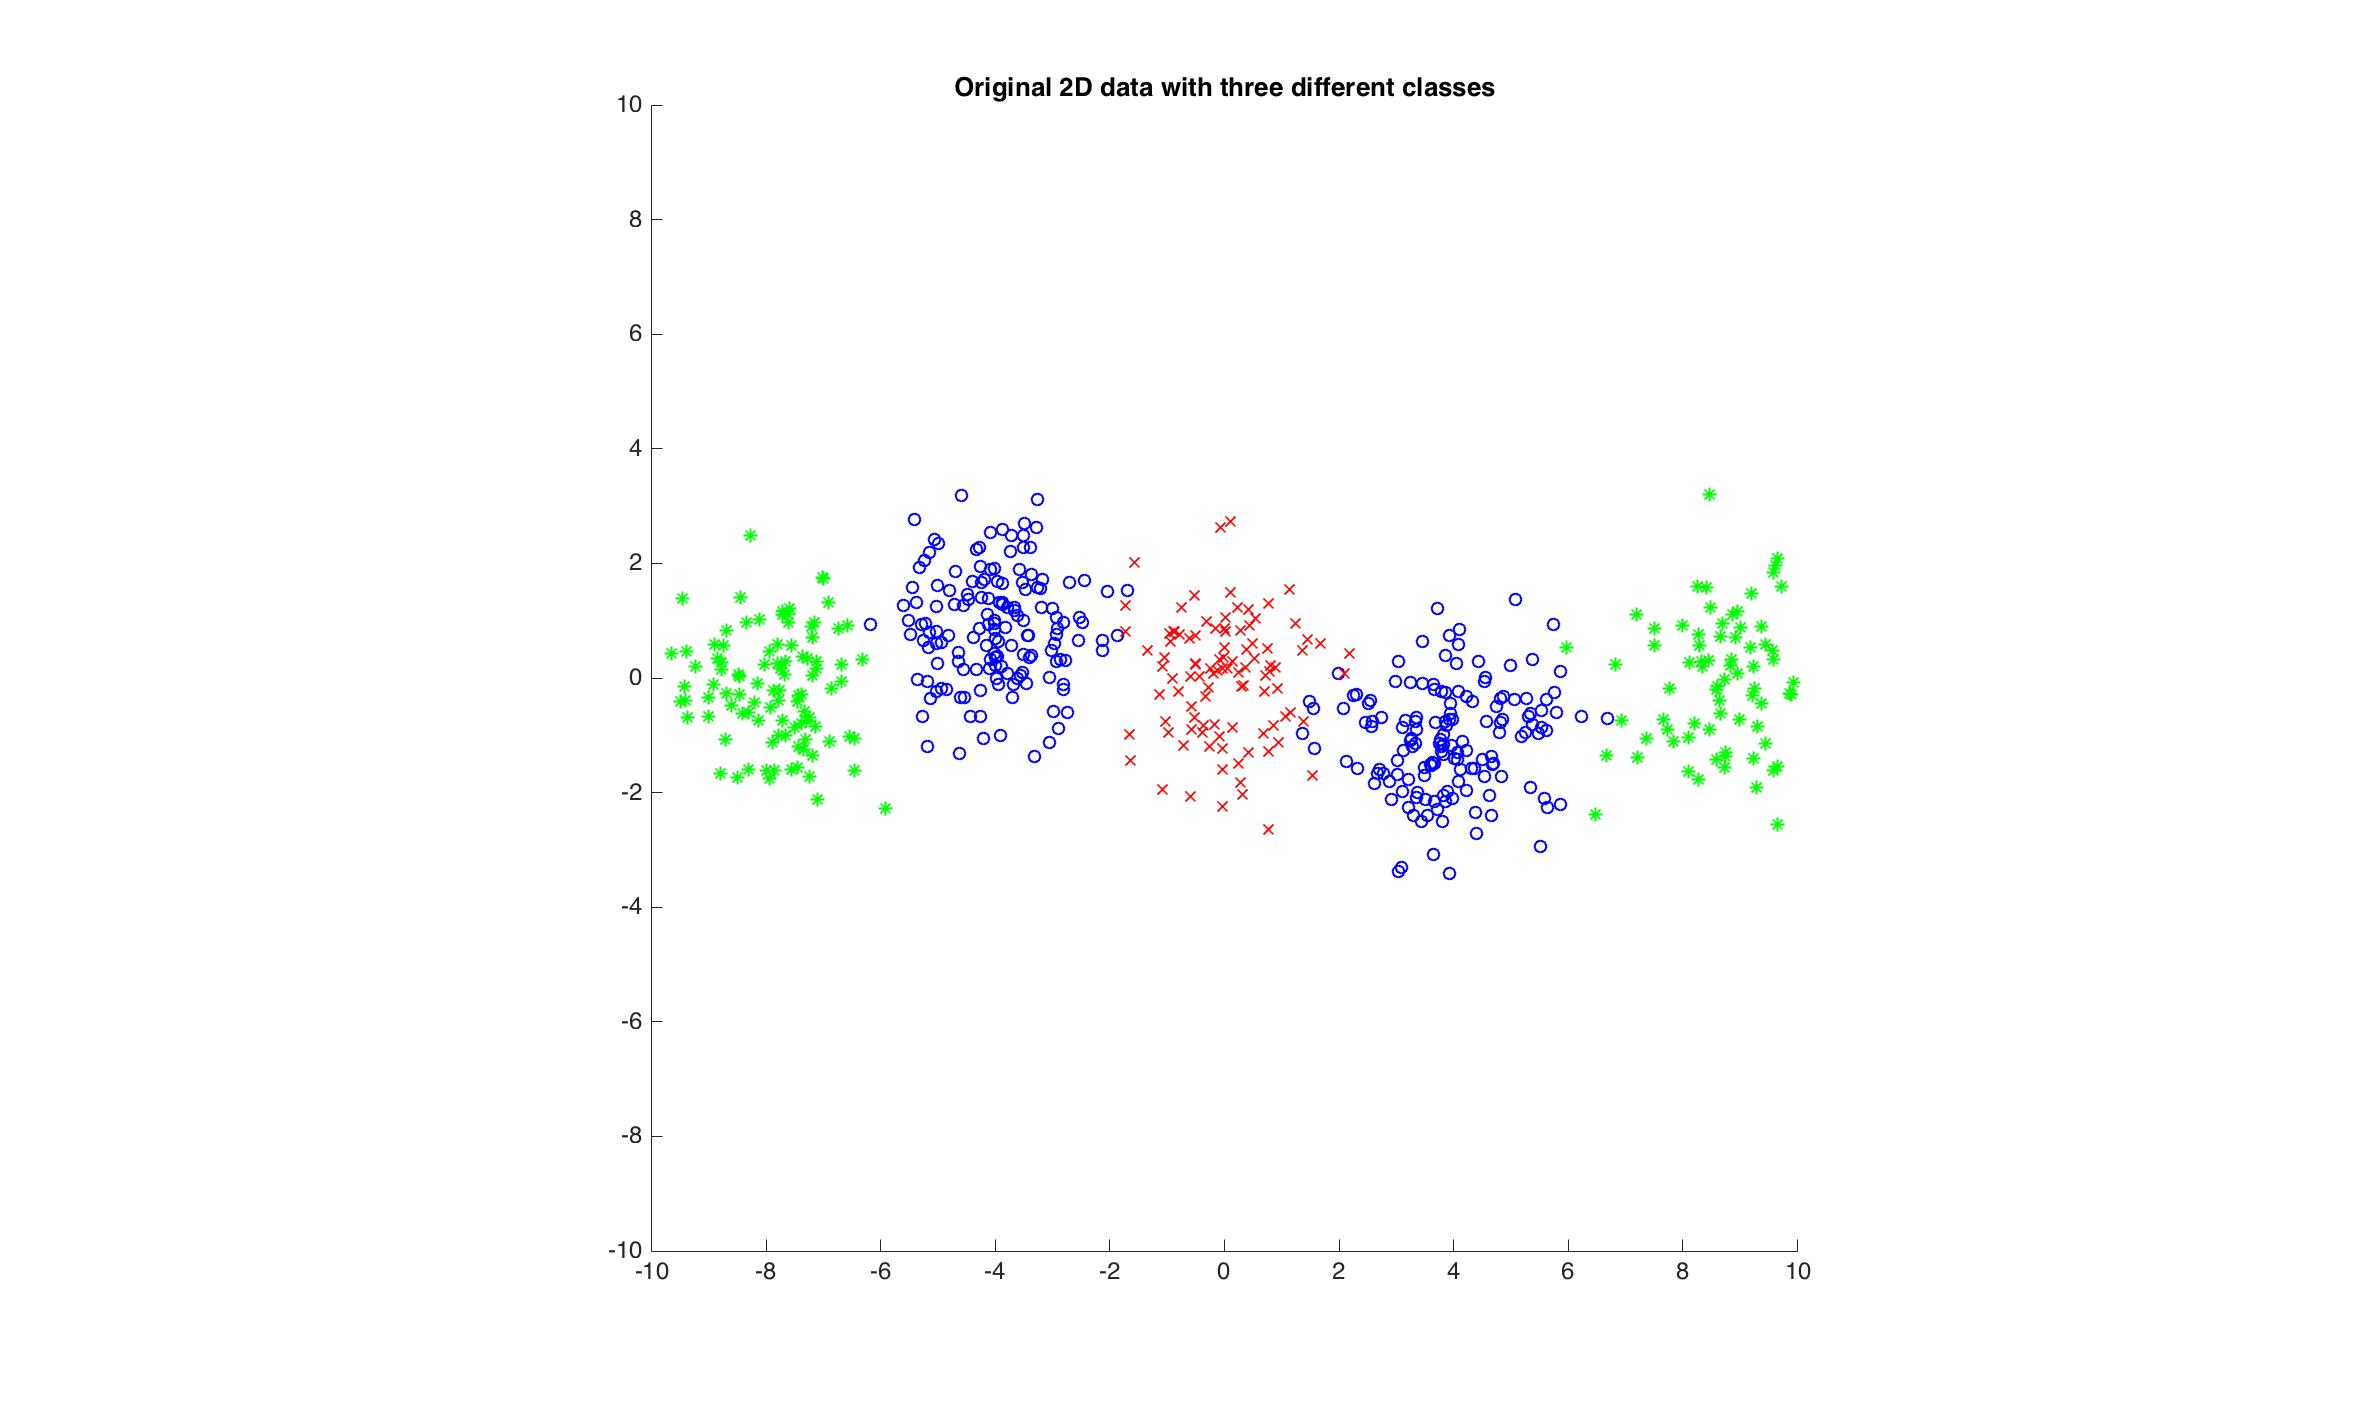
\includegraphics[width=1\linewidth]{/Users/JohnsonJohnson/Downloads/thesis_1/Figures/KLFDAdemo1.jpg}
%\caption{Example of five clusters belong to three classes}
%\vspace{0em}
%\end{figure} 
%\label{KLFDAdemo1}
%
%\begin{figure}[H]
%\centering
%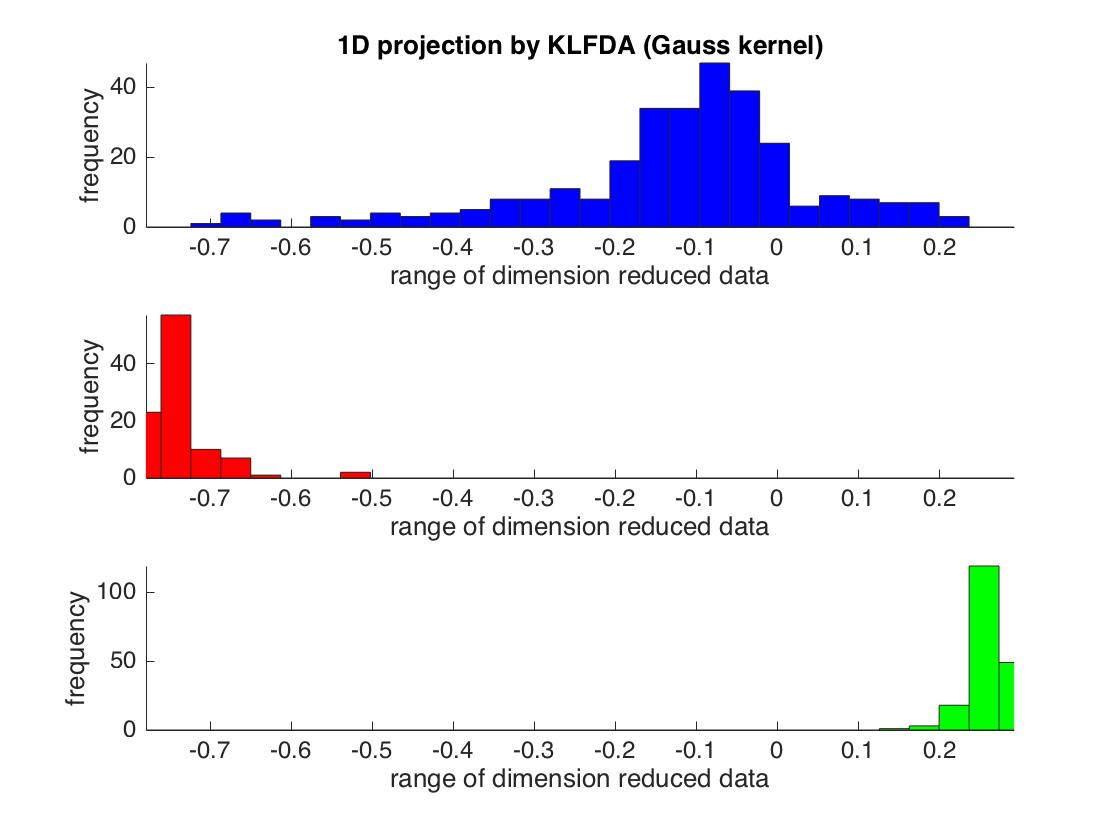
\includegraphics[width=1\linewidth]{/Users/JohnsonJohnson/Downloads/thesis_1/Figures/KLFDAdemo2.jpg}
%\caption{1-D distribution of dimension reduced data  with gaussian kernel}
%\vspace{-1em}
%\end{figure} 
%\label{KLFDAdemo2}
%
%\begin{figure}[H]
%\centering
%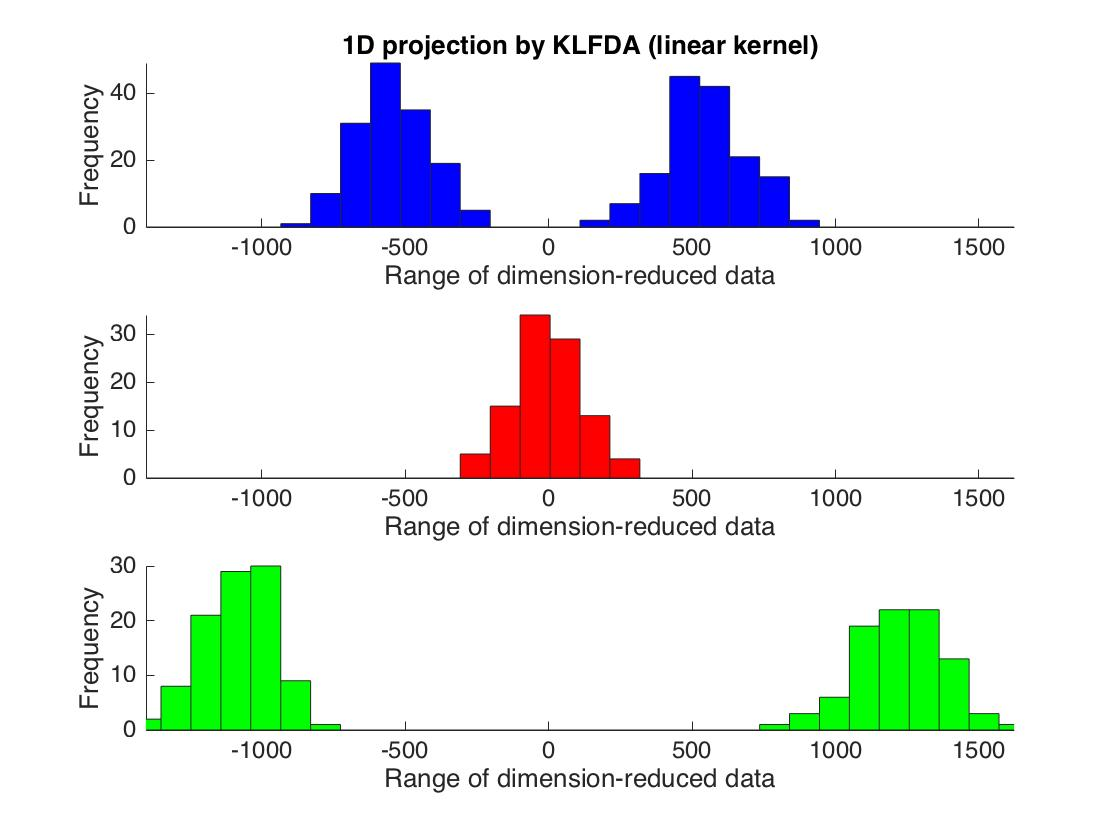
\includegraphics[width=1\linewidth]{/Users/JohnsonJohnson/Downloads/thesis_1/Figures/KLFDAdemo3.jpg}
%\caption{1-D distribution of dimension reduced data  with linear kernel}
%\vspace{-1em}
%\end{figure} 
%\label{KLFDAdemo3}
%%\begin{figure}[H]
%%\centering
%%\begin{minipage}[t]{0.5\linewidth}
%%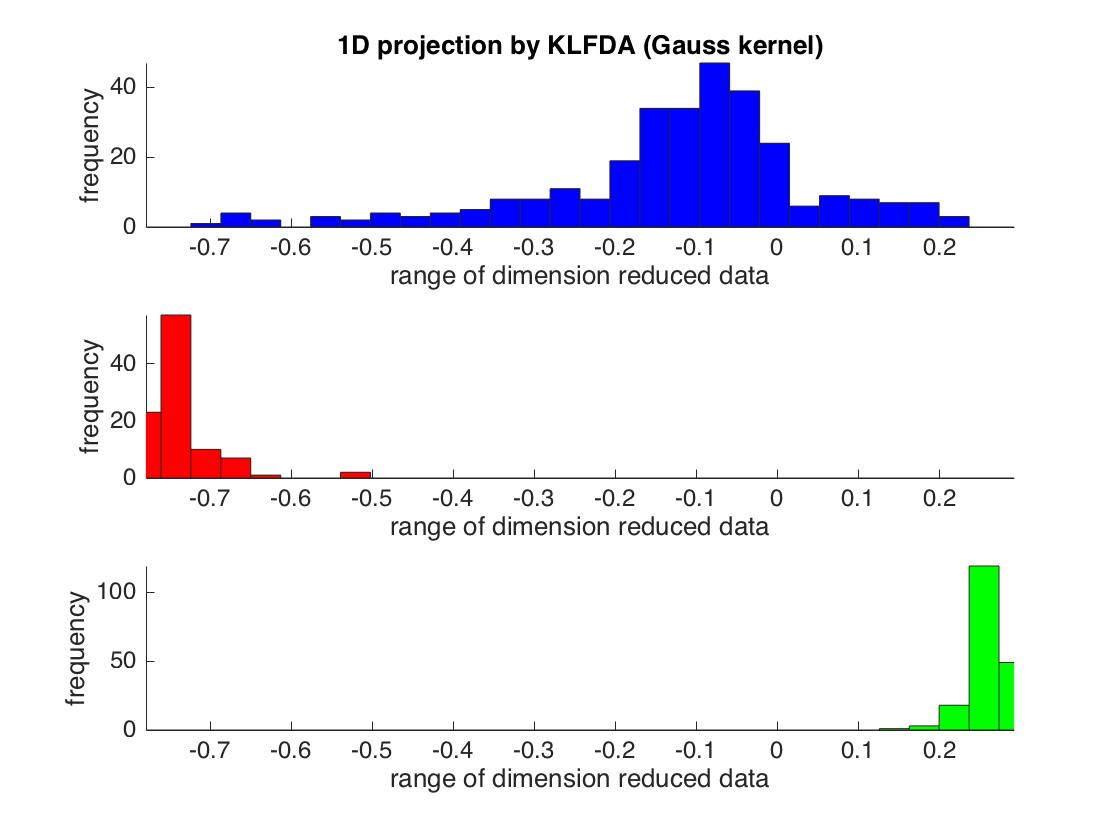
\includegraphics[width=2.7in]{/Users/JohnsonJohnson/Downloads/thesis_1/Figures/KLFDAdemo2.jpg}
%%%\caption{RGB patch}
%%\label{fig:side:a}
%%\end{minipage}%
%%\begin{minipage}[t]{0.5\linewidth}
%%\centering
%%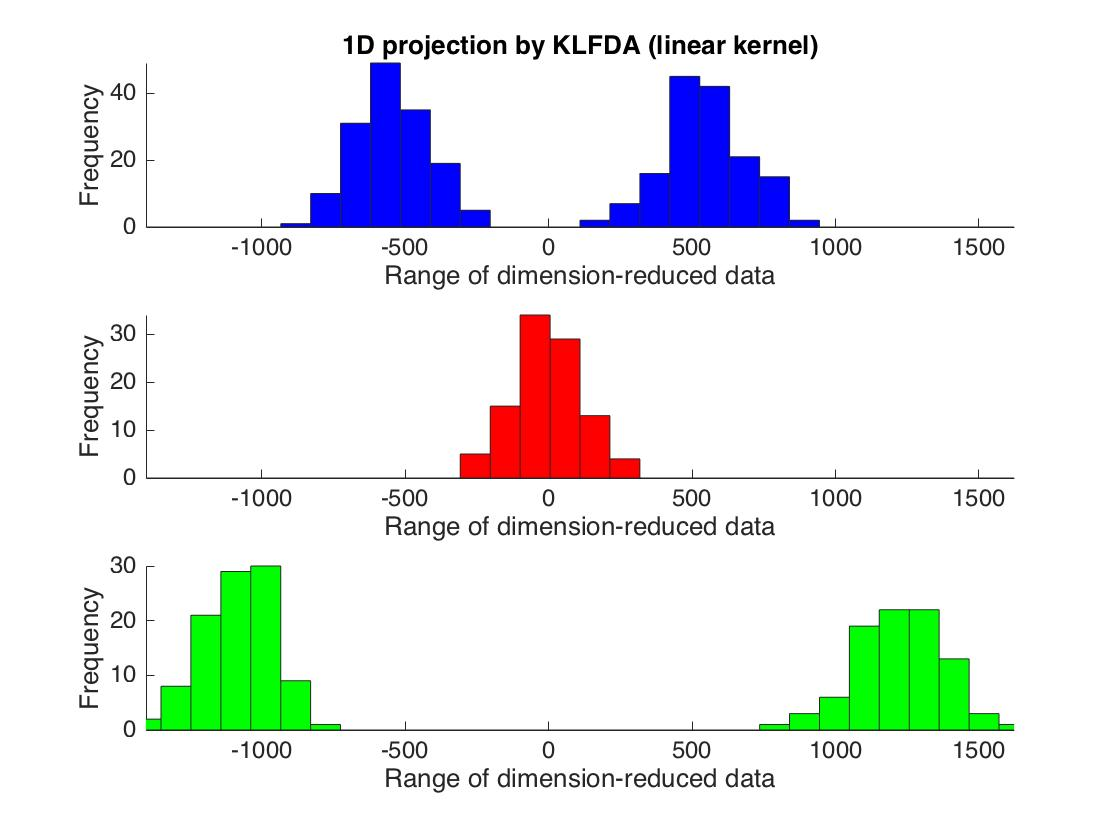
\includegraphics[width=2.7in]{/Users/JohnsonJohnson/Downloads/thesis_1/Figures/KLFDAdemo3.jpg}
%%%\caption{GBR patch}
%%\label{fig:side:b}
%%\end{minipage}
%%\caption{A comparison of two patches with same entropy but different color distribution}
%%\end{figure}
%
%
%
%
%
%
